% ============================================================
%  Chương: Kết quả và Đánh giá
%  Ước lượng lực từ biến dạng bề mặt cảm biến xúc giác
% ============================================================

\chapter{Kết quả và Đánh giá}
\label{chap:results}

Chương này trình bày kết quả thực nghiệm của ba hướng mô hình ước lượng lực
được đề xuất, bao gồm phân tích quá trình huấn luyện, đánh giá trên tập
kiểm thử và so sánh định lượng giữa các phương pháp.

% ============================================================
\section{Thiết lập thực nghiệm}
\label{sec:exp_setup}
% ============================================================

\subsection{Dữ liệu}

Dữ liệu thực nghiệm được thu thập từ hệ thống trạm thu thập đồng bộ gồm
camera xúc giác, cảm biến lực Imada~ZTA và cơ cấu động cơ tuyến tính điều
khiển qua Arduino. Mỗi mẫu là một cặp ảnh tham chiếu -- ảnh biến dạng kèm
nhãn lực (tính theo Newton) được lấy mẫu đồng thời.

Tập dữ liệu gồm \textbf{56 trial} đã được tiền xử lý và lưu dưới dạng cache.
Dữ liệu được phân chia theo đơn vị trial (không phải theo frame) để đánh giá
khả năng tổng quát hóa của mô hình trên các lần đo chưa xuất hiện trong quá
trình huấn luyện. Bảng~\ref{tab:dataset} tóm tắt phân phối tập dữ liệu.

\begin{table}[h]
\centering
\caption{Phân phối tập dữ liệu}
\label{tab:dataset}
\begin{tabular}{lc}
\toprule
\textbf{Thành phần} & \textbf{Giá trị} \\
\midrule
Tổng số trial & 56 \\
Trial train / validation / test & 39 / 8 / 9 \\
Số frame train & 11\,823 \\
Số frame validation & 3\,014 \\
Số frame test & 2\,660 \\
Thiết bị huấn luyện & CUDA (GPU) \\
\bottomrule
\end{tabular}
\end{table}

\subsection{Các mô hình so sánh}

Ba hướng tiếp cận được huấn luyện và đánh giá trên cùng tập dữ liệu:

\begin{itemize}
  \item \textbf{\texttt{force\_poly}} -- Hồi quy đa thức kết hợp MLP nhỏ.
        Đầu vào gồm 9 đặc trưng thủ công được trích xuất từ trường dịch
        chuyển marker (biên độ tối đa, độ lệch chuẩn, dịch chuyển trung bình
        theo trục, thành phần hướng kính và tiếp tuyến\ldots), sau đó được
        mở rộng bậc~2 thành 55 hạng đa thức. Đây là hướng tiếp cận nhẹ nhất,
        có khả năng diễn giải cao.

  \item \textbf{\texttt{force\_model}} -- Kiến trúc kiểu PointNet. Nhận trực
        tiếp tập marker đã qua tracking (tối đa 150 điểm), mỗi điểm mang vị
        trí chuẩn hóa và vector dịch chuyển. Shared~MLP kích thước (64, 128)
        trích xuất đặc trưng cục bộ, sau đó max-pooling tổng hợp toàn cục.
        Hướng tiếp cận này giữ lại cấu trúc không gian của trường biến dạng
        mà không cần ảnh đầy đủ.

  \item \textbf{\texttt{force\_cnn}} -- CNN end-to-end với backbone ResNet18
        pretrained. Đầu vào là cặp ảnh tham chiếu -- ảnh biến dạng đã resize
        về $240\times320$. Mô hình học trực tiếp từ thông tin thị giác, không
        phụ thuộc vào kết quả pipeline tracking.
\end{itemize}

\subsection{Chỉ số đánh giá}

Các chỉ số đánh giá sử dụng là:
\begin{itemize}
  \item \textbf{MAE} (Mean Absolute Error) -- sai số tuyệt đối trung bình;
  \item \textbf{RMSE} (Root Mean Squared Error) -- căn sai số bình phương
        trung bình, nhạy hơn với các sai lệch lớn;
  \item \textbf{R²} (hệ số xác định) -- tỷ lệ phương sai được giải thích bởi
        mô hình, lý tưởng bằng~1.
\end{itemize}

Checkpoint lưu là checkpoint có \textbf{MAE validation tốt nhất}, sau đó được
đánh giá trên tập test hoàn toàn độc lập.

% ============================================================
\section{Kết quả tổng quan}
\label{sec:overall_results}
% ============================================================

Bảng~\ref{tab:overall} tổng hợp kết quả của ba mô hình trên tập kiểm thử.

\begin{table}[h]
\centering
\caption{So sánh ba mô hình trên tập test (2\,660 frame, 9 trial)}
\label{tab:overall}
\begin{tabular}{lrrrrrrr}
\toprule
\textbf{Mô hình} & \textbf{\#Tham số} & \textbf{$t_\text{train}$ (s)}
  & \textbf{Val MAE*} & \textbf{Epoch*}
  & \textbf{Test MAE} & \textbf{Test RMSE} & \textbf{Test R²} \\
\midrule
\texttt{force\_poly}  &         913 &    31.8 & 0.0596 &  69 & 0.0680 & 0.1014 & 0.992 \\
\texttt{force\_model} &      25\,537 &    28.6 & 0.0517 &  34 & 0.0564 & 0.0798 & 0.995 \\
\texttt{force\_cnn}   & 11\,239\,169 & 1\,529.7 & 0.0310 &  57 & 0.0307 & 0.0405 & 0.999 \\
\bottomrule
\multicolumn{8}{l}{\footnotesize * Checkpoint tốt nhất được chọn theo MAE validation.}
\end{tabular}
\end{table}

Cả ba mô hình đều đạt R²~$>$~0.99, chứng tỏ cả ba đều học được quan hệ phi
tuyến giữa biến dạng bề mặt cảm biến và lực tác dụng. Trong đó,
\texttt{force\_cnn} đạt kết quả cao nhất với MAE~$=$~0.0307 và
R²~$=$~0.999. So với hai mô hình còn lại:

\begin{itemize}
  \item So với \texttt{force\_model}: CNN giảm MAE $\approx$~45.6\% và
        RMSE $\approx$~49.2\%.
  \item So với \texttt{force\_poly}: CNN giảm MAE $\approx$~54.9\% và
        RMSE $\approx$~60.1\%.
\end{itemize}

Tuy nhiên, cải thiện này đi kèm chi phí tính toán lớn hơn đáng kể:
\texttt{force\_cnn} có hơn 11,2 triệu tham số và cần khoảng 25,5 phút để
huấn luyện, trong khi \texttt{force\_poly} chỉ có 913 tham số và hoàn thành
trong 31,8 giây -- nhanh hơn khoảng \textbf{48 lần}.

% ============================================================
\section{Quá trình huấn luyện}
\label{sec:training_curves}
% ============================================================

\subsection{Polynomial Regression (\texttt{force\_poly})}

\begin{table}[h]
\centering
\caption{Tóm tắt quá trình huấn luyện \texttt{force\_poly}}
\label{tab:train_poly}
\begin{tabular}{ll}
\toprule
\textbf{Thuộc tính} & \textbf{Giá trị} \\
\midrule
Feature set & v1, 9 đặc trưng thủ công \\
Bậc đa thức & 2 \\
Số hạng đa thức & 55 \\
Head & MLP nhỏ (\texttt{mlp\_small}) \\
Số tham số & 913 \\
Early stopping & Sau 40 epoch không cải thiện \\
Val MAE epoch~1 / epoch tốt nhất & 0.1516 / 0.0596 \\
Train MAE epoch cuối & 0.0454 \\
Epoch tốt nhất / tổng & 69 / 109 \\
\bottomrule
\end{tabular}
\end{table}

Mô hình hội tụ rất nhanh: ngay từ epoch đầu tiên, R²~validation đã đạt
0.963. Sau khoảng 10 epoch, R²~validation dao động quanh 0.988--0.990 và
tiếp tục cải thiện chậm ở các epoch sau. Khoảng cách nhỏ giữa train MAE
(0.0454) và val MAE (0.0596) cho thấy mô hình khớp tốt mà không bị
over-fitting nghiêm trọng.

\subsection{ForceNet kiểu PointNet (\texttt{force\_model})}

\begin{table}[h]
\centering
\caption{Tóm tắt quá trình huấn luyện \texttt{force\_model}}
\label{tab:train_model}
\begin{tabular}{ll}
\toprule
\textbf{Thuộc tính} & \textbf{Giá trị} \\
\midrule
Số marker tối đa & 150 \\
Shared MLP & 64, 128 \\
Hidden head & 64, dropout~0.1 \\
Số tham số & 25\,537 \\
Early stopping & Sau 10 epoch không cải thiện \\
Val MAE epoch~1 / epoch tốt nhất & 0.3094 / 0.0517 \\
Train MAE epoch cuối & 0.1243 \\
Epoch tốt nhất / tổng & 34 / 44 \\
\bottomrule
\end{tabular}
\end{table}

Mô hình PointNet-style có val MAE epoch~1 cao hơn (0.3094) do bài toán phức
tạp hơn và số tham số nhiều hơn cần thời gian ổn định. Mô hình hội tụ nhanh
trong 34 epoch và dừng sớm vì không tiếp tục cải thiện. Khoảng cách
train/val MAE (0.1243 vs.\ 0.0826 tại epoch cuối) nhỏ, phản ánh khả năng
tổng quát hóa tốt.

\subsection{CNN End-to-End (\texttt{force\_cnn})}

\begin{table}[h]
\centering
\caption{Tóm tắt quá trình huấn luyện \texttt{force\_cnn}}
\label{tab:train_cnn}
\begin{tabular}{ll}
\toprule
\textbf{Thuộc tính} & \textbf{Giá trị} \\
\midrule
Backbone & ResNet18 pretrained \\
Kích thước ảnh đầu vào & $240 \times 320$ \\
Hidden head & 128, dropout~0.2 \\
Số tham số & 11\,239\,169 \\
Val MAE epoch~1 / epoch tốt nhất & 0.1778 / 0.0310 \\
Train MAE epoch cuối & 0.0815 \\
Epoch tốt nhất / tổng & 57 / 60 \\
\bottomrule
\end{tabular}
\end{table}

CNN cải thiện đều đặn trong suốt 60 epoch nhờ backbone pretrained đã mang
đặc trưng thị giác tốt từ ImageNet. Val MAE giảm từ 0.1778 (epoch~1) xuống
0.0310 (epoch~57), R²~validation đạt 0.9986 tại epoch cuối. Việc sử dụng
learning-rate scheduler giúp mô hình thoát khỏi cực tiểu cục bộ và tinh
chỉnh hiệu quả ở các epoch sau.

% ============================================================
\section{Kết quả chi tiết theo từng mô hình}
\label{sec:per_model_results}
% ============================================================

\subsection{Polynomial Regression (\texttt{force\_poly})}

Bảng~\ref{tab:poly_trial} trình bày kết quả của \texttt{force\_poly} trên 9
trial kiểm thử.

\begin{table}[h]
\centering
\caption{Kết quả từng trial -- \texttt{force\_poly}}
\label{tab:poly_trial}
\begin{tabular}{lrrrr}
\toprule
\textbf{Trial} & \textbf{Số frame} & \textbf{MAE} & \textbf{RMSE} & \textbf{R²} \\
\midrule
\texttt{s1/trial\_008} & 159 & 0.0512 & 0.0840 & 0.996 \\
\texttt{2/trial\_009}  & 420 & 0.0410 & 0.0547 & 0.998 \\
\texttt{t1/trial\_009} & 142 & 0.0755 & 0.1077 & 0.993 \\
\texttt{1/trial\_003}  & 361 & 0.0589 & 0.0707 & 0.992 \\
\texttt{s1/trial\_001} & 334 & 0.1020 & 0.1556 & 0.981 \\
\texttt{c1/trial\_008} & 140 & 0.0720 & 0.1031 & 0.992 \\
\texttt{1/trial\_002}  & 316 & 0.1335 & 0.1584 & 0.971 \\
\texttt{2/trial\_008}  & 462 & 0.0353 & 0.0543 & 0.998 \\
\texttt{2/trial\_003}  & 326 & 0.0639 & 0.0905 & 0.995 \\
\midrule
\textbf{Tổng / TB} & \textbf{2\,660} & \textbf{0.0680} & \textbf{0.1014} & \textbf{0.992} \\
\bottomrule
\end{tabular}
\end{table}

Mô hình đạt kết quả tốt trên phần lớn trial, nhưng sai số tăng rõ ở
\texttt{1/trial\_002} (MAE~$=$~0.1335) và \texttt{s1/trial\_001}
(MAE~$=$~0.1020). Điều này cho thấy đặc trưng tổng hợp 9~chiều có giới hạn
khi điều kiện tiếp xúc hoặc phân bố biến dạng khác biệt so với phần lớn dữ
liệu huấn luyện.

Một ưu điểm quan trọng của \texttt{force\_poly} là \textbf{khả năng diễn
giải}. Các hệ số lớn nhất trong mô hình (Bảng~\ref{tab:coeff}) liên quan đến
biên độ dịch chuyển cực đại (\texttt{disp\_mag\_max}, hệ số~1.09), độ lệch
chuẩn dịch chuyển (\texttt{disp\_mag\_std}, 0.50) và dịch chuyển trung bình
theo trục~$x$ (\texttt{dx\_mean}, $-$0.37). Điều này phù hợp với trực giác
vật lý: lực lớn làm tăng biên độ biến dạng đồng thời thay đổi phân bố không
gian của trường dịch chuyển.

\begin{table}[h]
\centering
\caption{Năm hệ số lớn nhất -- \texttt{force\_poly}}
\label{tab:coeff}
\begin{tabular}{lr}
\toprule
\textbf{Đặc trưng} & \textbf{Hệ số} \\
\midrule
\texttt{disp\_mag\_max}           &  1.094 \\
bias (hệ số tự do)               &  0.717 \\
\texttt{disp\_mag\_std}           &  0.496 \\
\texttt{dx\_mean}                 & $-$0.370 \\
\texttt{radial\_disp\_mean}       & $-$0.235 \\
\bottomrule
\end{tabular}
\end{table}

\subsection{ForceNet kiểu PointNet (\texttt{force\_model})}

Bảng~\ref{tab:model_trial} trình bày kết quả của \texttt{force\_model}.

\begin{table}[h]
\centering
\caption{Kết quả từng trial -- \texttt{force\_model}}
\label{tab:model_trial}
\begin{tabular}{lrrrr}
\toprule
\textbf{Trial} & \textbf{Số frame} & \textbf{MAE} & \textbf{RMSE} & \textbf{R²} \\
\midrule
\texttt{s1/trial\_008} & 159 & 0.0678 & 0.0931 & 0.995 \\
\texttt{2/trial\_009}  & 420 & 0.0463 & 0.0691 & 0.996 \\
\texttt{t1/trial\_009} & 142 & 0.0764 & 0.0979 & 0.994 \\
\texttt{1/trial\_003}  & 361 & 0.0491 & 0.0685 & 0.992 \\
\texttt{s1/trial\_001} & 334 & 0.0691 & 0.0953 & 0.993 \\
\texttt{c1/trial\_008} & 140 & 0.0532 & 0.0716 & 0.996 \\
\texttt{1/trial\_002}  & 316 & 0.0694 & 0.0910 & 0.990 \\
\texttt{2/trial\_008}  & 462 & 0.0442 & 0.0641 & 0.997 \\
\texttt{2/trial\_003}  & 326 & 0.0564 & 0.0827 & 0.996 \\
\midrule
\textbf{Tổng / TB} & \textbf{2\,660} & \textbf{0.0564} & \textbf{0.0798} & \textbf{0.995} \\
\bottomrule
\end{tabular}
\end{table}

So với \texttt{force\_poly}, \texttt{force\_model} cải thiện đáng kể trên
các trial khó. Cụ thể, tại \texttt{1/trial\_002}, MAE giảm từ 0.1335 xuống
0.0694 ($-$48\%); tại \texttt{s1/trial\_001}, MAE giảm từ 0.1020 xuống
0.0691 ($-$32\%). Điều này chứng minh rằng biểu diễn theo tập marker giúp
mô hình xử lý tốt hơn các trường hợp phân bố biến dạng phức tạp, vốn không
được nắm bắt đầy đủ bởi 9 đặc trưng tổng hợp.

\subsection{CNN End-to-End (\texttt{force\_cnn})}

Bảng~\ref{tab:cnn_trial} trình bày kết quả của \texttt{force\_cnn}.

\begin{table}[h]
\centering
\caption{Kết quả từng trial -- \texttt{force\_cnn}}
\label{tab:cnn_trial}
\begin{tabular}{lrrrr}
\toprule
\textbf{Trial} & \textbf{Số frame} & \textbf{MAE} & \textbf{RMSE} & \textbf{R²} \\
\midrule
\texttt{s1/trial\_008} & 159 & 0.0374 & 0.0526 & 0.998 \\
\texttt{2/trial\_009}  & 420 & 0.0249 & 0.0332 & 0.999 \\
\texttt{t1/trial\_009} & 142 & 0.0369 & 0.0532 & 0.998 \\
\texttt{1/trial\_003}  & 361 & 0.0245 & 0.0333 & 0.998 \\
\texttt{s1/trial\_001} & 334 & 0.0333 & 0.0391 & 0.999 \\
\texttt{c1/trial\_008} & 140 & 0.0431 & 0.0595 & 0.997 \\
\texttt{1/trial\_002}  & 316 & 0.0354 & 0.0428 & 0.998 \\
\texttt{2/trial\_008}  & 462 & 0.0254 & 0.0336 & 0.999 \\
\texttt{2/trial\_003}  & 326 & 0.0339 & 0.0412 & 0.999 \\
\midrule
\textbf{Tổng / TB} & \textbf{2\,660} & \textbf{0.0307} & \textbf{0.0405} & \textbf{0.999} \\
\bottomrule
\end{tabular}
\end{table}

Sai số của CNN không chỉ thấp hơn về trung bình mà còn \textbf{ổn định hơn
giữa các trial}: MAE trải từ 0.0245 đến 0.0431, khoảng dao động là 0.0186.
Trong khi đó, \texttt{force\_poly} có khoảng dao động 0.0982 và
\texttt{force\_model} là 0.0322. Điều này cho thấy backbone ResNet18 khai
thác được các tín hiệu biến dạng mà pipeline marker có thể làm mất trong quá
trình phát hiện, tracking và rút gọn đặc trưng.

% ============================================================
\section{So sánh định lượng giữa ba mô hình}
\label{sec:comparison}
% ============================================================

\subsection{So sánh MAE theo từng trial}

Bảng~\ref{tab:mae_comparison} đặt MAE của ba mô hình cạnh nhau trên từng
trial kiểm thử.

\begin{table}[h]
\centering
\caption{So sánh MAE theo trial trên tập test}
\label{tab:mae_comparison}
\begin{tabular}{lrrrr}
\toprule
\textbf{Trial} & \textbf{\texttt{force\_poly}} & \textbf{\texttt{force\_model}}
  & \textbf{\texttt{force\_cnn}} & \textbf{Tốt nhất} \\
\midrule
\texttt{s1/trial\_008} & 0.0512 & 0.0678 & \textbf{0.0374} & \texttt{force\_cnn} \\
\texttt{2/trial\_009}  & 0.0410 & 0.0463 & \textbf{0.0249} & \texttt{force\_cnn} \\
\texttt{t1/trial\_009} & 0.0755 & 0.0764 & \textbf{0.0369} & \texttt{force\_cnn} \\
\texttt{1/trial\_003}  & 0.0589 & 0.0491 & \textbf{0.0245} & \texttt{force\_cnn} \\
\texttt{s1/trial\_001} & 0.1020 & 0.0691 & \textbf{0.0333} & \texttt{force\_cnn} \\
\texttt{c1/trial\_008} & 0.0720 & 0.0532 & \textbf{0.0431} & \texttt{force\_cnn} \\
\texttt{1/trial\_002}  & 0.1335 & 0.0694 & \textbf{0.0354} & \texttt{force\_cnn} \\
\texttt{2/trial\_008}  & 0.0353 & 0.0442 & \textbf{0.0254} & \texttt{force\_cnn} \\
\texttt{2/trial\_003}  & 0.0639 & 0.0564 & \textbf{0.0339} & \texttt{force\_cnn} \\
\midrule
\textbf{Trung bình} & 0.0680 & 0.0564 & \textbf{0.0307} & \texttt{force\_cnn} \\
\bottomrule
\end{tabular}
\end{table}

\texttt{force\_cnn} là mô hình tốt nhất trên \textbf{cả 9/9 trial} kiểm thử.
\texttt{force\_model} đứng thứ hai trên 6/9 trial, đặc biệt cải thiện rõ so
với \texttt{force\_poly} ở các trial có sai số lớn.

\subsection{Đánh đổi độ chính xác -- chi phí tính toán}

Hình~\ref{fig:tradeoff} minh họa mối quan hệ giữa số lượng tham số và hiệu
năng mô hình (Test MAE). Ba mô hình thể hiện ba điểm đánh đổi rõ ràng:

\begin{itemize}
  \item \texttt{force\_poly} (913 tham số, MAE~$=$~0.068): phù hợp với
        thiết bị hạn chế tài nguyên, yêu cầu tốc độ suy luận cao hoặc cần
        khả năng giải thích mô hình.
  \item \texttt{force\_model} (25\,537 tham số, MAE~$=$~0.056): cân bằng
        giữa độ chính xác và chi phí tính toán; không yêu cầu ảnh đầy đủ,
        chỉ cần kết quả tracking.
  \item \texttt{force\_cnn} (11,2~M tham số, MAE~$=$~0.031): độ chính xác
        cao nhất nhưng yêu cầu GPU để huấn luyện trong thời gian hợp lý.
\end{itemize}

\begin{figure}[h]
  \centering
  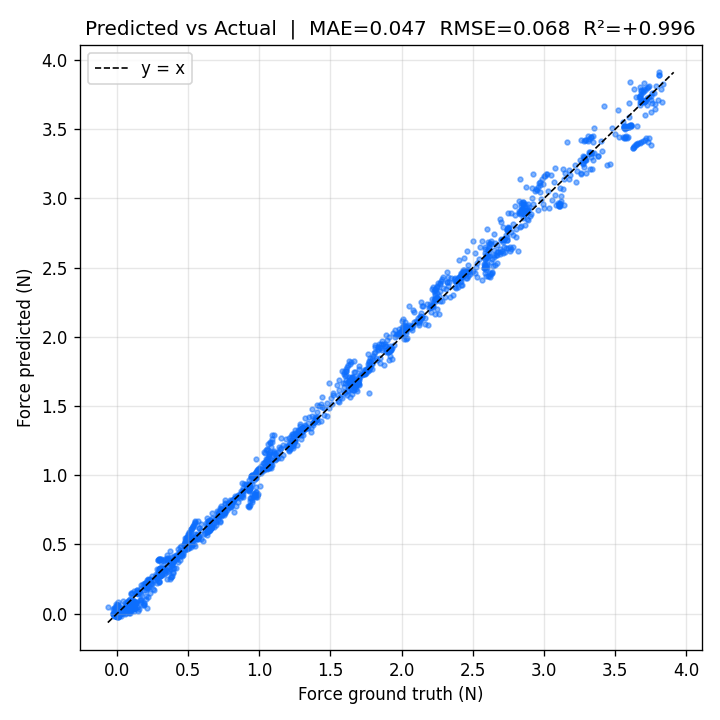
\includegraphics[width=0.45\textwidth]{outputs/force_poly/eval/test_scatter.png}
  \hfill
  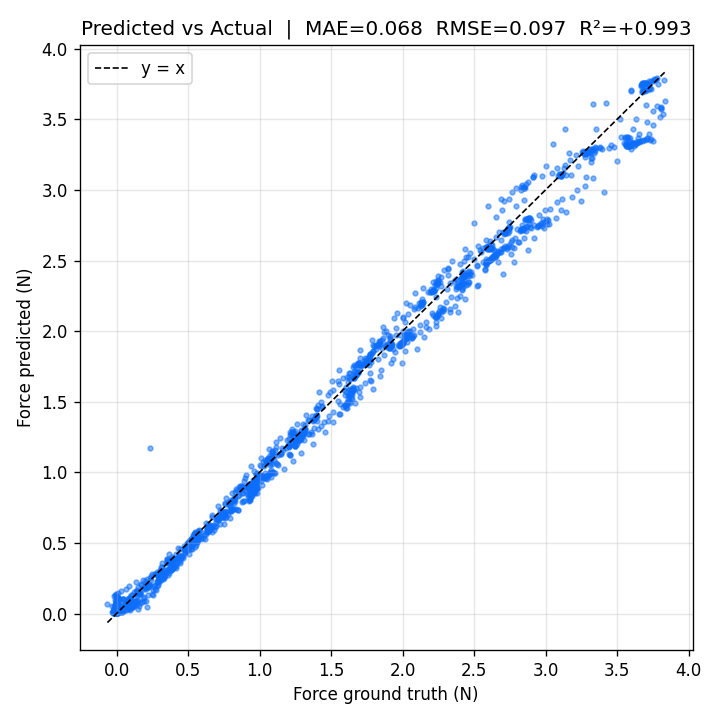
\includegraphics[width=0.45\textwidth]{outputs/force_model/eval/test_scatter.png}
  \caption{Scatter plot dự đoán -- nhãn thật trên tập test.
           Trái: \texttt{force\_poly}. Phải: \texttt{force\_model}.}
  \label{fig:scatter_12}
\end{figure}

\begin{figure}[h]
  \centering
  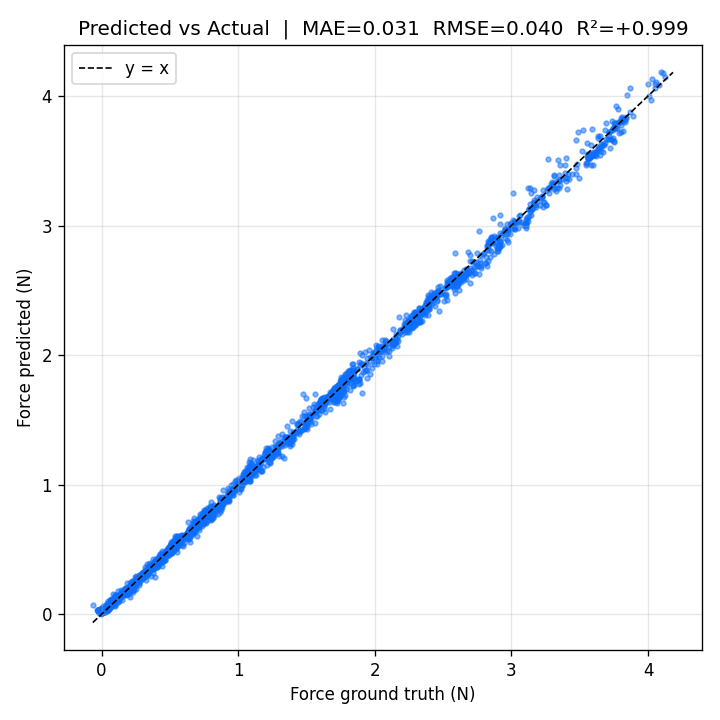
\includegraphics[width=0.55\textwidth]{outputs/force_cnn/eval/test_scatter.png}
  \caption{Scatter plot dự đoán -- nhãn thật trên tập test: \texttt{force\_cnn}.
           Các điểm bám sát đường $y=x$ cho thấy R²~$=$~0.999.}
  \label{fig:scatter_cnn}
\end{figure}

\begin{figure}[h]
  \centering
  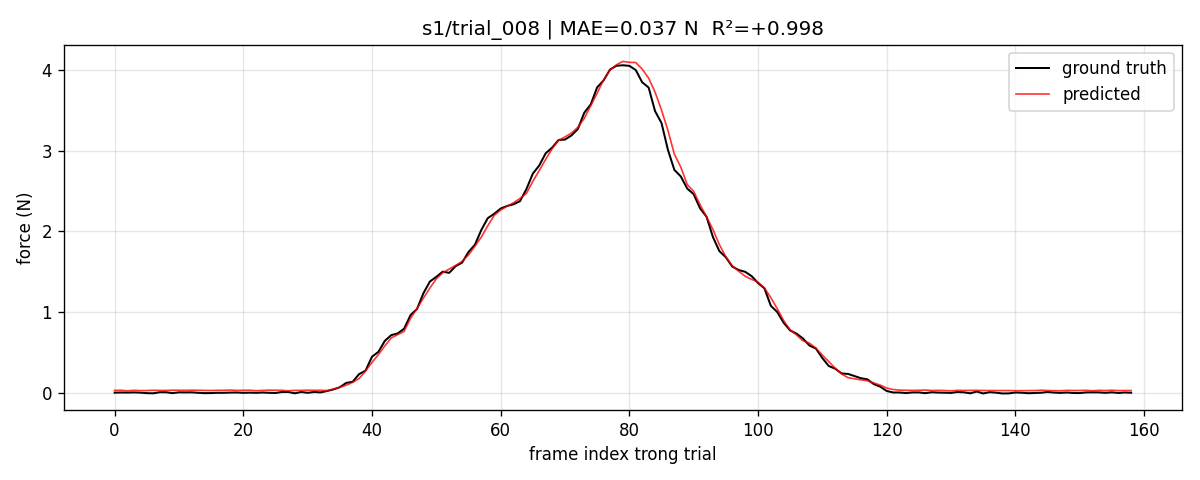
\includegraphics[width=0.95\textwidth]{outputs/force_cnn/eval/test_timeseries_trial0.png}
  \caption{Chuỗi thời gian dự đoán của \texttt{force\_cnn} trên một trial
           kiểm thử điển hình. Đường liền: giá trị thật. Đường đứt: dự đoán.}
  \label{fig:timeseries_cnn}
\end{figure}

% ============================================================
\section{Phân tích và thảo luận}
\label{sec:discussion}
% ============================================================

\subsection{Ảnh hưởng của mức độ trừu tượng đầu vào}

Kết quả thực nghiệm cho thấy mức độ thông tin đầu vào ảnh hưởng trực tiếp
đến chất lượng dự đoán lực, theo xu hướng: \emph{đặc trưng tổng hợp $\to$
tập điểm $\to$ ảnh thô} ứng với độ chính xác tăng dần.

\textbf{\texttt{force\_poly}} tổng hợp toàn bộ trường dịch chuyển thành 9
số. Bước rút gọn này mất nhiều thông tin không gian, đặc biệt khi phân bố
biến dạng không đồng đều hoặc bất đối xứng -- điều thường xảy ra khi vật thể
tiếp xúc ở rìa cảm biến. Dù vậy, 9 đặc trưng đủ phản ánh lực trong đa số
trường hợp (R²~$=$~0.992) và ưu điểm diễn giải giúp gỡ lỗi và phân tích
phụ thuộc đặc trưng dễ dàng.

\textbf{\texttt{force\_model}} giữ lại cấu trúc theo từng marker, cho phép
mô hình học phân bố không gian của biến dạng. Đây là lý do mô hình xử lý tốt
hơn các trial khó (như \texttt{1/trial\_002}). Tuy nhiên, chất lượng đầu vào
phụ thuộc vào pipeline phát hiện và tracking marker. Nếu marker bị mất hoặc
phân bố không đều do ánh sáng không ổn định, sai số có thể tăng.

\textbf{\texttt{force\_cnn}} học trực tiếp từ ảnh, không bị giới hạn bởi
chất lượng tracking. Backbone ResNet18 pretrained trích xuất đặc trưng thị
giác phong phú từ gradient và cấu trúc biến dạng ở nhiều tầng không gian.
Đây là lý do mô hình đạt sai số thấp và ổn định trên toàn bộ trial kiểm
thử. Nhược điểm chính là yêu cầu bộ nhớ và tính toán cao trong quá trình
huấn luyện.

\subsection{Tính ổn định giữa các trial}

Một kết quả đáng chú ý là sự khác biệt về \emph{tính ổn định} giữa ba mô
hình. Bảng~\ref{tab:stability} trình bày độ lệch chuẩn của MAE trên 9 trial
kiểm thử.

\begin{table}[h]
\centering
\caption{Tính ổn định MAE giữa các trial kiểm thử}
\label{tab:stability}
\begin{tabular}{lrrr}
\toprule
\textbf{Mô hình} & \textbf{MAE trung bình} & \textbf{MAE max} & \textbf{MAE min} \\
\midrule
\texttt{force\_poly}  & 0.0680 & 0.1335 & 0.0353 \\
\texttt{force\_model} & 0.0564 & 0.0764 & 0.0442 \\
\texttt{force\_cnn}   & 0.0307 & 0.0431 & 0.0245 \\
\bottomrule
\end{tabular}
\end{table}

\texttt{force\_cnn} có khoảng dao động MAE nhỏ nhất (0.0186), trong khi
\texttt{force\_poly} có khoảng dao động lớn nhất (0.0982). Điều này cho thấy
CNN không chỉ tốt hơn về trung bình mà còn \emph{đáng tin cậy hơn} khi gặp
các điều kiện tiếp xúc mới.

\subsection{Hướng cải tiến}

Dựa trên kết quả trên, một số hướng cải tiến có thể được xem xét:

\begin{itemize}
  \item \textbf{Tăng kích thước dữ liệu}: 56 trial với ~17\,500 frame là
        tương đối nhỏ cho một mô hình CNN 11,2~M tham số. Việc thu thập thêm
        dữ liệu với nhiều loại vật thể và điều kiện tiếp xúc đa dạng có thể
        cải thiện thêm khả năng tổng quát hóa.

  \item \textbf{Knowledge distillation}: Chuyển tri thức từ \texttt{force\_cnn}
        sang mô hình nhẹ hơn để kết hợp ưu điểm tốc độ của
        \texttt{force\_poly} và độ chính xác của CNN.

  \item \textbf{Ensemble}: Kết hợp dự đoán từ \texttt{force\_model} và
        \texttt{force\_poly} có thể cải thiện tính ổn định mà không tăng quá
        nhiều chi phí suy luận.

  \item \textbf{Uncertainty estimation}: Bổ sung ước lượng độ không chắc
        chắn (ví dụ: MC Dropout) để mô hình tự báo cáo khi dự đoán không
        đáng tin cậy.
\end{itemize}

% ============================================================
\section{Kết luận chương}
\label{sec:chapter_conclusion}
% ============================================================

Chương này đã trình bày và so sánh ba hướng tiếp cận ước lượng lực từ biến
dạng bề mặt cảm biến xúc giác. Kết quả thực nghiệm trên 2\,660 frame từ 9
trial kiểm thử cho thấy:

\begin{enumerate}
  \item \textbf{Cả ba mô hình đều khả thi}: R²~$>$~0.99 chứng tỏ quan hệ
        giữa biến dạng hình ảnh và lực tác dụng có thể được học hiệu quả bằng
        nhiều cấp độ biểu diễn khác nhau.

  \item \textbf{\texttt{force\_cnn} đạt kết quả tốt nhất}: MAE~$=$~0.0307,
        RMSE~$=$~0.0405 và R²~$=$~0.999 trên tập test, ổn định trên toàn bộ
        trial. Đây là mô hình phù hợp khi yêu cầu độ chính xác cao nhất.

  \item \textbf{\texttt{force\_model} là lựa chọn trung gian hiệu quả}:
        MAE~$=$~0.0564 và R²~$=$~0.995, tốt hơn mô hình đa thức 17\% về MAE,
        chỉ cần 25\,537 tham số và không yêu cầu ảnh đầy đủ.

  \item \textbf{\texttt{force\_poly} là baseline hữu ích}: Chỉ 913 tham số,
        huấn luyện trong 31,8~giây, có khả năng diễn giải qua hệ số đặc trưng,
        phù hợp với thiết bị hạn chế tài nguyên hoặc khi cần phân tích nhân
        quả.
\end{enumerate}

Ba mô hình phản ánh ba mức đánh đổi rõ ràng giữa \emph{độ chính xác},
\emph{chi phí tính toán} và \emph{khả năng diễn giải}, tạo thành một phổ
lựa chọn phù hợp với nhiều bối cảnh triển khai khác nhau trong robotics xúc
giác.
